% !TEX TS-program = xelatex
% !TEX encoding = UTF-8 Unicode
% !Mode:: "TeX:UTF-8"

\documentclass{resume}
\usepackage{zh_CN-Adobefonts_external} % Simplified Chinese Support using external fonts (./fonts/zh_CN-Adobe/)
% \usepackage{NotoSansSC_external}
% \usepackage{NotoSerifCJKsc_external}
% \usepackage{zh_CN-Adobefonts_internal} % Simplified Chinese Support using system fonts
\usepackage{linespacing_fix} % disable extra space before next section
\usepackage{cite}
\usepackage{comment}

\usepackage{tabularx}
\usepackage{multirow}
\usepackage[absolute,overlay]{textpos}  % 用于绝对定位
\usepackage{ulem}

\begin{document}
\pagenumbering{gobble} % suppress displaying page number


\begin{comment}
\begin{table}[]
\begin{tabular}{ll}
\scshape{陆嘉琛}                                              & \multirow{6}{*}{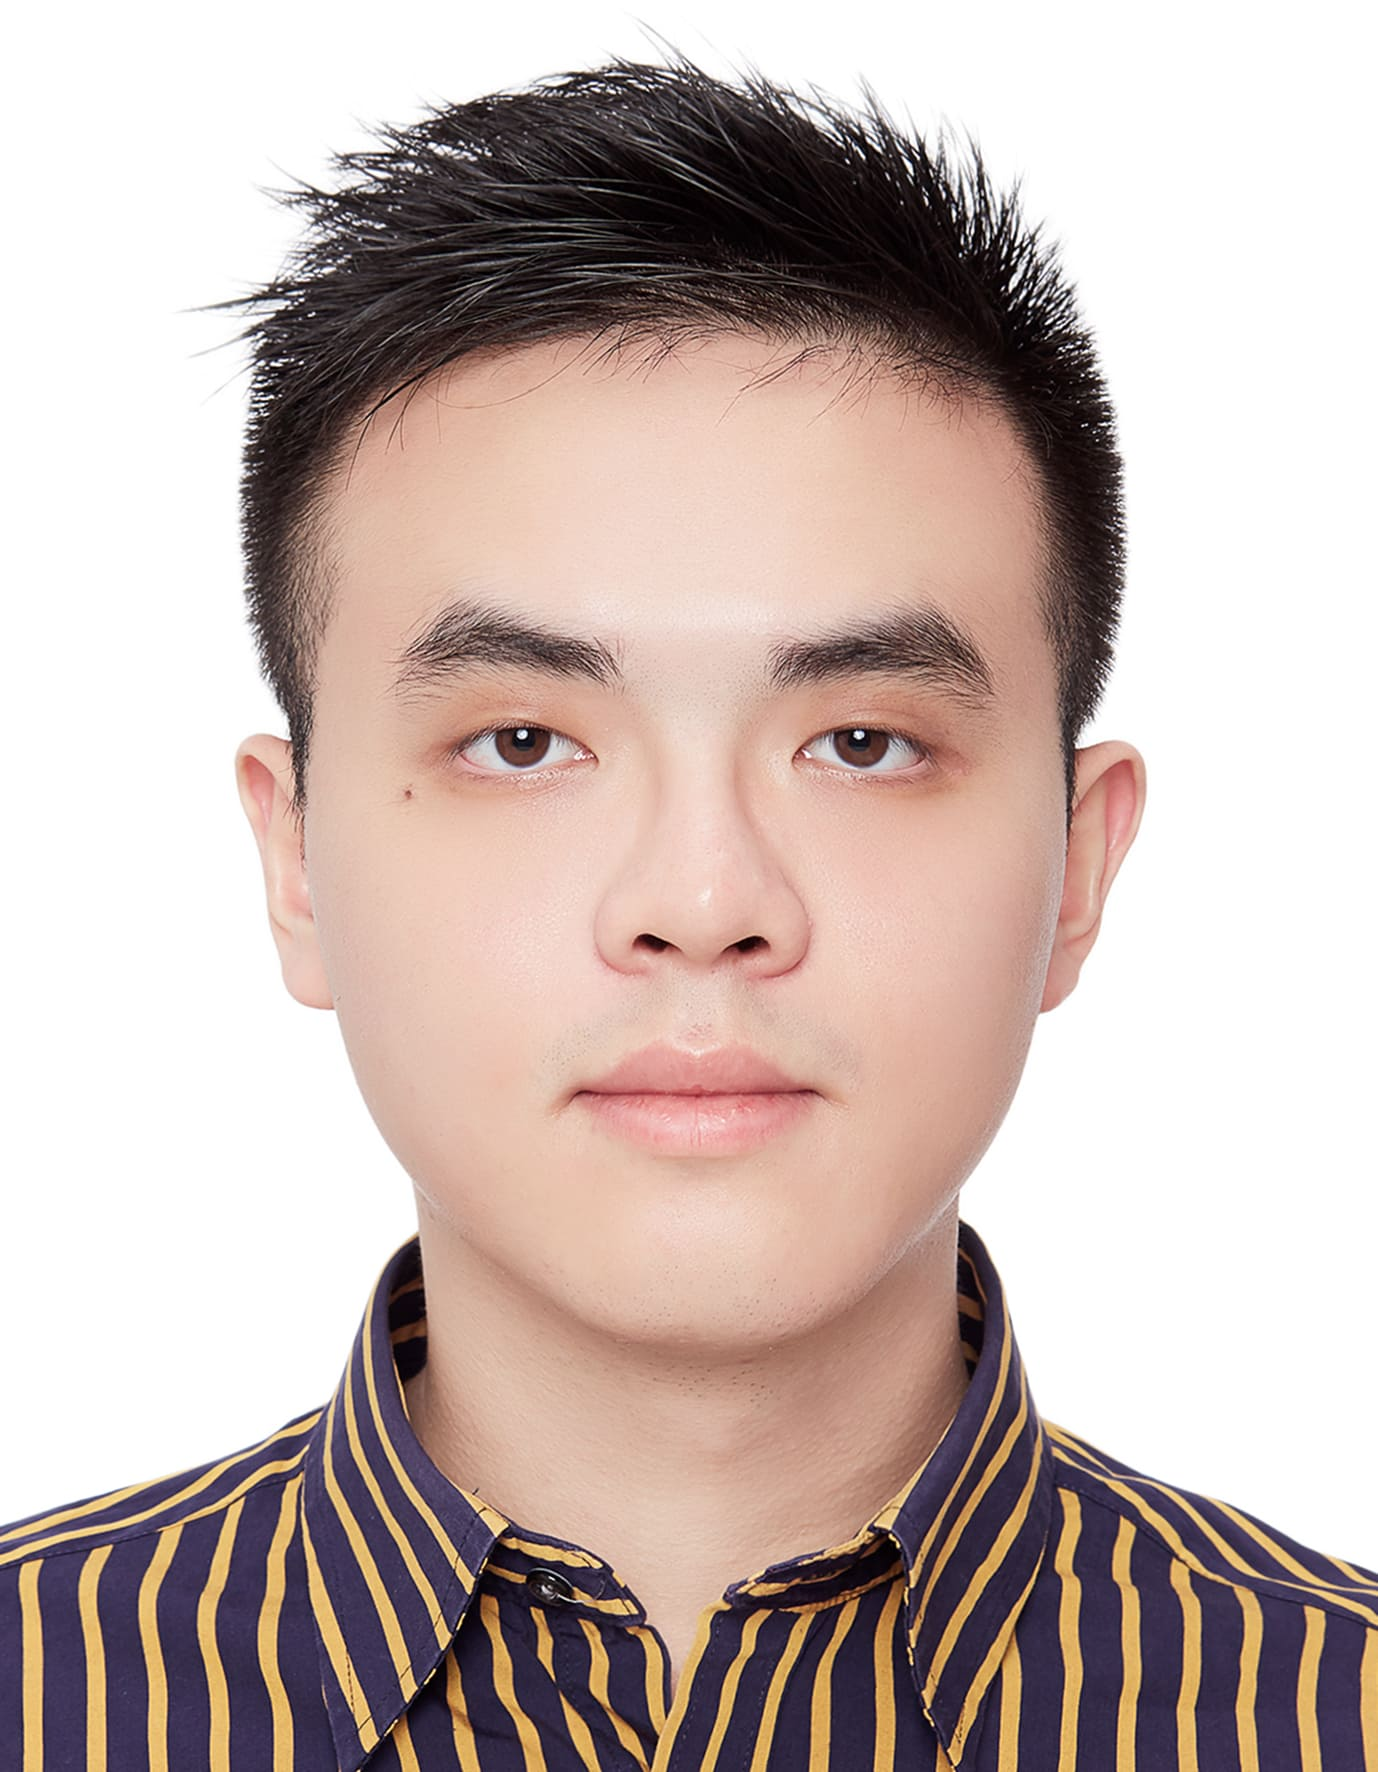
\includegraphics[width=3cm]{Max.jpg}} \\
\email{jiachen\_lu1999@163.com}                                   &                                                                               \\
\phone{(+86) 139-1860-2264}                                     &                                                                               \\
\linkedin[Jiachen Lu]{https://www.linkedin.com/in/jiachen-lu-08b85a1bb/}     &                                                                              \\
\github[github.com/Jiachen Lu]{https://github.com/LuckyMax0722}       &                                                                               \\
\homepage[homepage/Jiachen Lu]{https://luckymax0722.github.io/}                                                   &                                                                              

\end{tabular}
\end{table}


\name{陆嘉琛}

\basicInfo{
  \email{jiachen\_lu1999@163.com} \textperiodcentered\ 
  \phone{(+86) 139-1860-2264} \textperiodcentered\ 
  \linkedin[Jiachen Lu]{https://www.linkedin.com/in/jiachen-lu-08b85a1bb/} \textperiodcentered\ 
  \github[Jiachen Lu]{https://github.com/LuckyMax0722} \textperiodcentered\ 
  \homepage[Jiachen Lu]{https://luckymax0722.github.io/}
}
\end{comment}

\name{陆嘉琛}

\basicInfo{
  \email{jiachen\_lu1999@163.com} \textperiodcentered\ 
  \phone{(+86) 139-1860-2264} \textperiodcentered\ 
  \linkedin[Linkedin.com/Jiachen Lu]{https://www.linkedin.com/in/jiachen-lu-08b85a1bb/}
}

\basicInfo{
  \github[Github.com/Jiachen Lu]{https://github.com/LuckyMax0722} \textperiodcentered\ 
  \homepage[\sout{Homepage.com/Jiachen Lu}]{https://luckymax0722.github.io/}
}


\begin{textblock*}{3cm}(17cm,0cm)  % 3cm是图片宽度,(16cm,1cm)是图片左上角的位置
    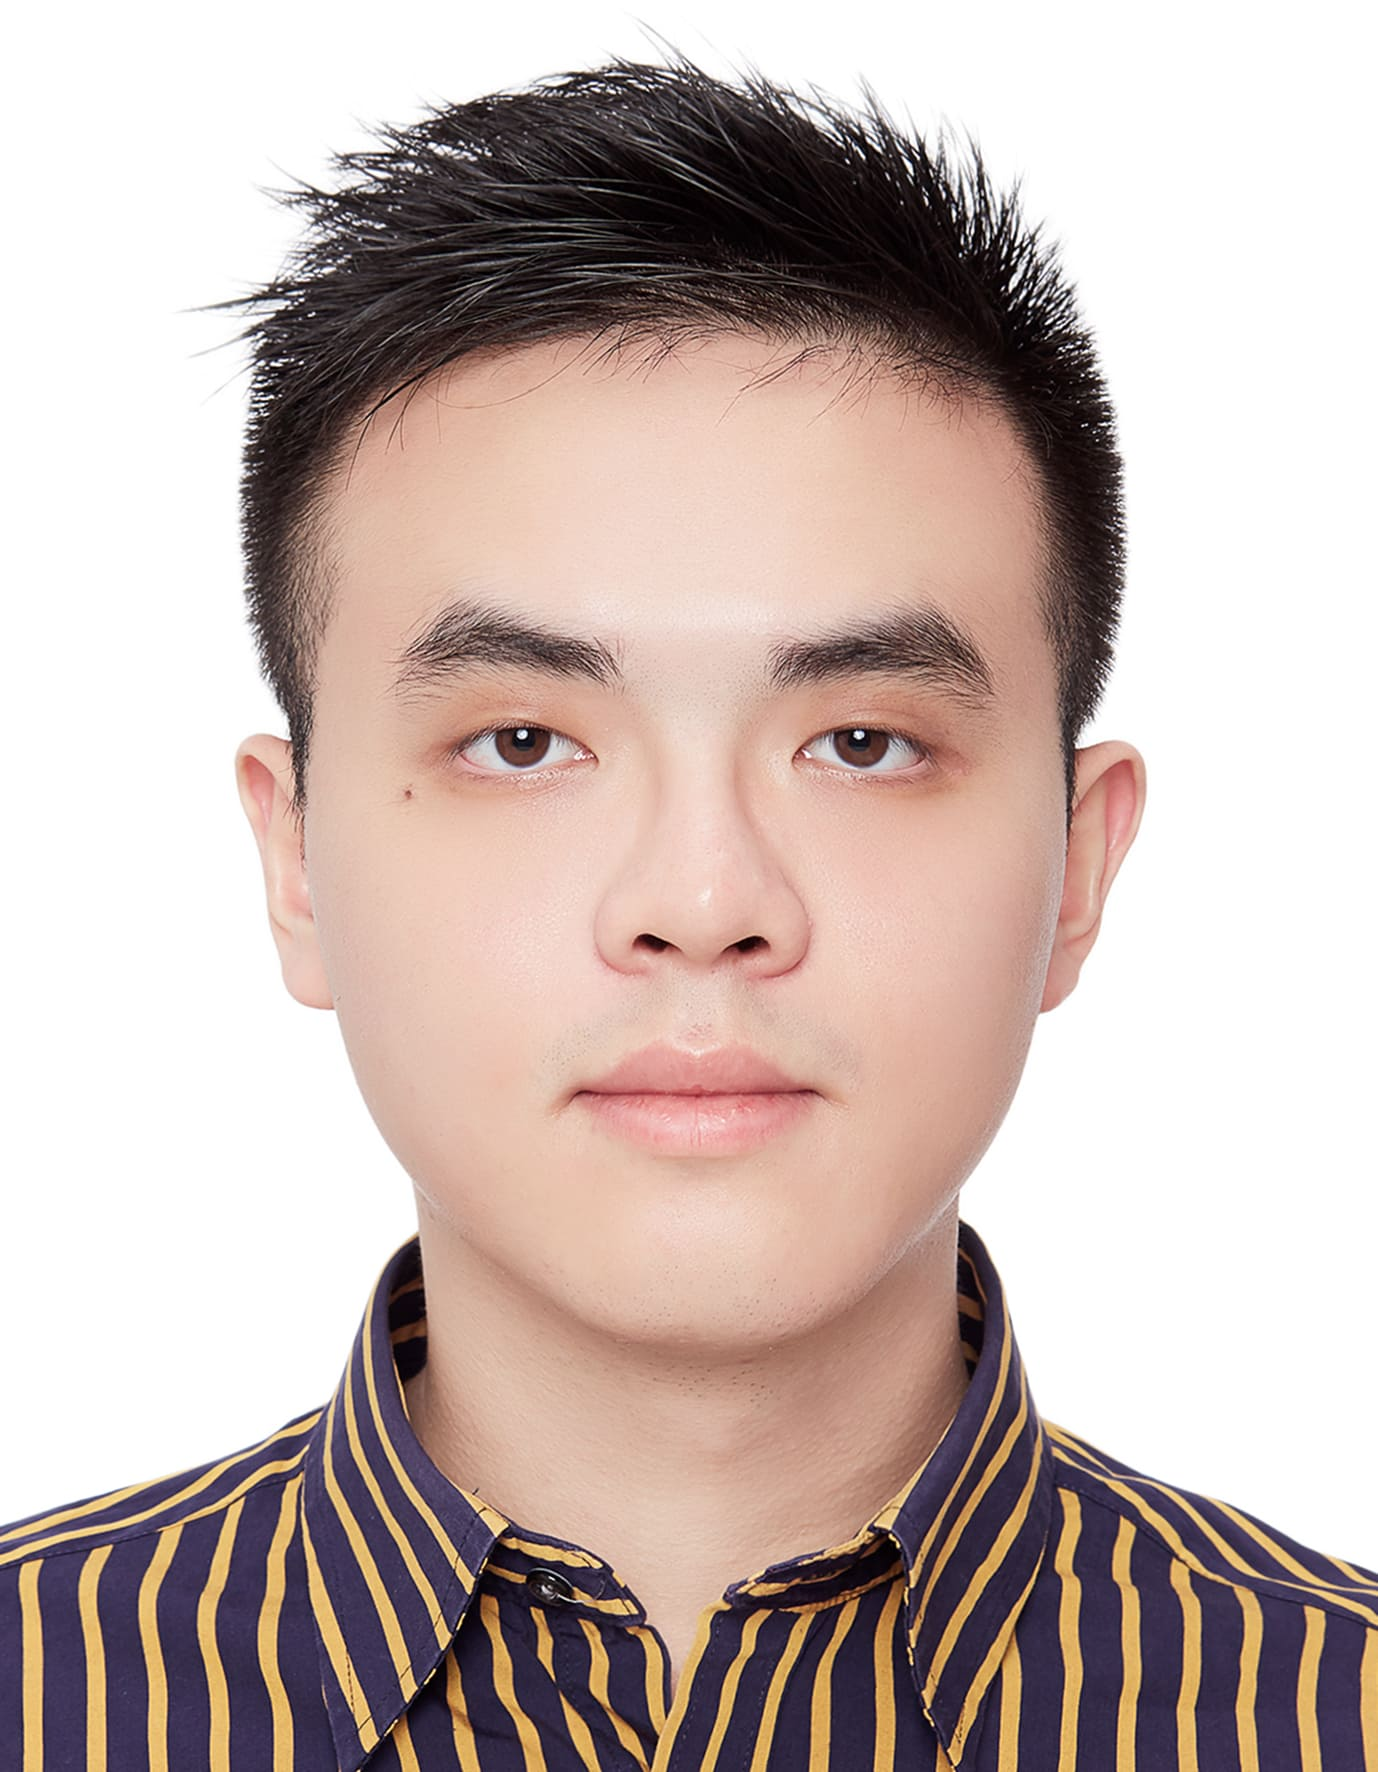
\includegraphics[width=2.6cm]{Max.jpg}  % 替换为你的图片路径
\end{textblock*}

\section{\faGraduationCap\  教育背景}
\edusubsection
  {\textbf{慕尼黑工业大学}, 慕尼黑, 德国}
  {\textbf{机器人,认知,智能}\ |\ \textit{理学硕士(M.Sc.)}}
  {2022.10—2025.06}
  \gpasubsection{核心课程:}{人工智能, 机器人, 机器学习,机器学习(图和序列数据), 深度学习}{GPA: 91/100}
  \gpasubsection{}{计算机视觉(多视角几何/检测、分割和跟踪), 驾驶辅助系统, 自动驾驶软件开发等}{}
\vspace{0.1cm}

\edusubsection
  {\textbf{科堡应用技术大学}, 科堡, 德国}
  {\textbf{车辆工程}\ |\ \textit{工学学士(B.Eng.)}}
  {2020.10—2022.04}
  \gpasubsection{核心课程:}{车辆动力学, 机电一体化等}{GPA: 87/100}
\vspace{0.1cm}

\edusubsection
  {\textbf{同济大学}, 上海, 中国}
  {\textbf{车辆服务工程}\ |\ \textit{工学学士(B.Eng.)}}
  {2017.10—2022.04}
  \gpasubsection{核心课程:}{高等数学, 大学物理, 力学, 电学, 控制理论, 车辆工程,传感器与执行器等}{GPA: 80/100}
\vspace{0.1cm}

\section{\faUsers\ 工作经历}
\worksubsection{\textbf{保时捷工程服务公司}, 门斯海姆, 德国}{\textbf{ADAS测试开发工程师}\ |\ \textit{实习}}{2024.04—2024.09}
\ \textit{技术栈:\ Python/PyTorch/PyTorch Lightning/Jira/Confluence/Codebeamer}
\begin{itemize}
  \item 支持人工智能团队的日常工作,完成单目相机三维场景重建相关的子任务。基于\textbf{LATR},一种3D车道线检测模型,实现了推理和可视化的脚本,用于检测和分类道路边界和围栏。基于\textbf{SignParser}复现了项目的部分代码,用于识别和理解基于文本的交通标志。复现了\textbf{Metric3D},一种用于重建三维交通标志的模型。整合上述模型的输出,并在模拟器中实时生成真实世界的三维模型
  \item 负责Mobileye SuperVision的L2++级辅助驾驶系统(ADAS)的功能/单元/整合测试。基于Google Map和实际驾驶经历构建测试参考路线,并基于多维度测试评估矩阵和实际天气及道路状况设计测试案例
  \item 为配备IAV和博世泊车辅助系统的Macan 4提供测试系统维护和开发,并为ePark/TPA/RA等功能测试提供现场支持和陪同测试,实时记录测试状态和测试案例通过情况。并基于 \textbf{YOLOv9}开发用于检测人机界面(HMI)按钮状态的视频检测模型,用于与 CAN-BUS 上的按钮信号进行比对。
  \item 支持ADAS驾驶和泊车团队日常的开发和测试工作,并负责ADAS团队新入职员工的入职培训
\end{itemize}
\vspace{0.1cm}

\worksubsection{\textbf{戴姆勒卡车公司}, 斯图加特, 德国}{\textbf{充电系统测试开发工程师}\ |\ \textit{学士论文}}{2021.10—2022.03}
\ \textit{论文题目:\ 开发用于研究充电系统控制单元和软件模块的残余总线模拟以及测试概念}

\ \textit{技术栈:\ CAPL/Vector CANoe/Hardware-in-the-loop(HiL)/
Restbussimulation}
\begin{itemize}
  \item 设计并开发用于eActros电动卡车充电系统组件测试的V模型,\textbf{硬件在环模拟(HiL)}和\textbf{残余总线模拟}
  \item 基于现有的测试框架和ECU的开发标准,编写,优化和扩展现有的测试框架和测试用例
  \item 引入关键绩效指标(KPI)概念,开发用于测试用例自动化的评估标准和工具,并对现有的测试用例进行评估
  \item 基于CAPL和CANoe编写自动化测试用例的实施脚本,设计并构建相应的脚本配置以及可视化的用户操作界面
\end{itemize}
\vspace{0.1cm}

\worksubsection{\textbf{戴姆勒卡车公司}, 埃斯林根, 德国}{\textbf{高压组件测试开发工程师}\ |\ \textit{实习}}{2021.05—2021.10}
\ \textit{技术栈:\ CAPL/Vector CANape/Vector CANalyzer}
\begin{itemize}
  \item 支持全球团队日常开发和测试eActros电动卡车动力系统中的高压电阻组件
  \item 为eActros的夏季道路功能测试提供测试概念的设计和测试计划的协调,并在测试期间提供现场支持和陪同测试
  \item 基于CANape设计并构建可视化的图形用户界面(GUI),用于实时监控测试车辆特定组件的运行状态。并编写组件测试脚本,通过监控CAN-Bus实现来实现测试数据的监测,收集和在线分析
  \item 基于CAPL和CANape的数据挖掘功能,开发并编写用于离线评估测试车辆特定组件的\textbf{自动化数据挖掘脚本}
\end{itemize}
\vspace{0.1cm}

\section{\faFolder\ 项目经历}
\projsubsection{\textbf{硕士论文: 基于单目相机的3D语义场景补全}}{2024.08—2025.06}
\ \textit{技术栈:\ Python/Pytorch \hfill 项目链接:\ }
\begin{itemize}
  \item 基于\textbf{MonoScene}和\textbf{VoxFormer}的开发
\end{itemize}
\vspace{0.1cm}

\projsubsection{\textbf{TOD2D: 2D图像的道路物体目标检测和分类}}{2024.03—2024.07}
\ \textit{技术栈:\ Python/Pytorch/OpenCV/YOLOv5-v9/DETR/SwinT/ResNet/EfficientNet \hfill 项目链接:\ \href{https://github.com/LuckyMax0722/TOD2D}{TOD2D}}
\begin{itemize}
  \item 基于nuImages的2D驾驶图像数据集,进行数据清洗,数据扩增和\textbf{YOLO/COCO}格式的数据集的创建
  \item 利用属于One-Stage的\textbf{YOLOv5-v9}和基于Transformer的\textbf{DETR/SwinT}对nuImages数据集中的图像实现目标检测
  \item 利用\textbf{OpenCV}和预训练的\textbf{YOLOv9}对红绿灯数据集\textbf{DTLD/BSTLD}以及交通标志数据集\textbf{GTSRB/TT100K}进行目标物体的提取和预分类,重新调整目标物体的图片大小并创建YOLO格式的数据集
  \item 利用手动创建的红绿灯和交通标志数据集,基于\textbf{ResNet50}和\textbf{EfficientNet b3}预训练用于细分红绿灯种类和颜色的分类头和用于细分交通标志种类和内容的分类头,并将其作为\textbf{YOLOv9}的Second-Stage分类器
  \item 相较于直接训练\textbf{YOLOv9},\textbf{TOD}的训练速度提高了\textbf{65\%},硬件需求降低了\textbf{25\%}并且ACC提高了约\textbf{12\%}
\end{itemize}
\vspace{0.1cm}

\projsubsection{\textbf{端到端学习的自动驾驶汽车}}{2023.10—2024.03}
\ \textit{技术栈:\ Python/Pytorch/Pytorch Lightening/OpenCV/ResNet/ViT/GRU \hfill 项目链接:\ \href{https://github.com/LuckyMax0722/SelfDrivingCars}{SelfDrivingCars}}
\begin{itemize}
  \item 基于Unity的汽车驾驶模拟器,手动采样训练数据,并利用\textbf{OpenCV库}对原始图像数据进行清洗,筛选,处理及扩增
  \item 利用\textbf{ResNet50}作为图像特征学习骨干模块,实现利用车辆前方图像直接预测转向角的功能,即端到端学习
  \item 在消融实验中,测试了不同的网络架构在实现端到端学习的表现,包括\textbf{ResNet50},\textbf{ResNet50+GRU以}及\textbf{ViT}等
  \item 相比较于其他模型,ResNet50的训练和推理速度提高了\textbf{35\%},并且基于ResNet50训练的自动驾驶模型实现了小车在驾驶模拟器中\textbf{0}碰撞的高速行驶
\end{itemize}
\vspace{0.1cm}

\projsubsection{\textbf{SoftCap: 利用稀疏卷积模块为3D点云场景生成密集描述}}{2023.04—2023.09}
\ \textit{技术栈:\ Python/Pytorch/Pytorch Lightening/C++/SoftGroup/GNN/GRU/Attention \hfill 项目链接:\ \href{https://github.com/LuckyMax0722/SoftCap}{SoftCap}}
\begin{itemize}
  \item 在3D点云场景中应用\textbf{SoftGroup}作为检测骨干模块,对点云数据实施软分组机制,以实现实例提案的生成和分类
  \item 基于3D点云场景中实例之间的物理关系构建\textbf{GNN},并通过消息传递算法来获取并学习实例与实例间的空间特征
  \item 基于增强的物体特征,通过多层\textbf{GRU模块和注意力机制}来生成3D点云场景中实例特征及其空间属性的描述
  \item 在训练模型的过程中,使用了基于\textbf{Teacher Forcing}的监督学习和基于\textbf{Self-Critical}的强化学习
  \item 在ScanRefer数据集中,SoftCap在定位和描述3D点云场景中的物体时表现良好,\textbf{mAP@0.5IoU}达到了\textbf{57.38},\textbf{CIDEr@0.5IoU}达到了\textbf{36.27}。 与之前的工作相比,SoftCap的性能提高了 \textbf{140\%}
\end{itemize}
\vspace{0.1cm}

\section{\faStar\ 奖项}

\begin{itemize}
  \item \itemsubsection{\textbf{菲尼克斯奖学金}}{}{}{}{}{}{}{获得时间: 2020.09}
\end{itemize}
\vspace{0.1cm}

\section{\faCogs\ IT 技能}
\begin{itemize}
  \item \textbf{编程语言:} Python, C++, CAPL, Matlab/Simulink
  \item \textbf{常用工具:} Pytorch, Pytorch Lightening, NumPy, OpenCV, mm-toolkit, Pandas, Git, Docker
  \item \textbf{常用软件:} Word/Excel/PowerPoint, Vector CANoe/CANape/CANalyzer, AutoCAD, CATIA V5
\end{itemize}
\vspace{0.1cm}

\section{\faLanguage\ 语言能力}
% increase linespacing [parsep=0.5ex]
\begin{itemize}
  \item \itemsubsection{\textbf{英语(C1):}}{雅思(IELTS)}
  {总分:7}{听力:8}{阅读:7}{写作:6.5}{口语:6}{获得成绩时间: 2022.01}

  \itemsubsection{\textbf{}}{CET4}
  {总分:586}{}{}{}{}{获得成绩时间: 2018.06}

  \itemsubsection{\textbf{}}{CET6}
  {总分:466}{}{}{}{}{获得成绩时间: 2018.12}

  \vspace{0.1cm}
  \item \itemsubsection{\textbf{德语(C1):}}{德福(TestDaF)}
  {总分:15}{听力:3}{阅读:4}{写作:4}{口语:4}{获得成绩时间: 2021.12}
\end{itemize}
\vspace{0.1cm}

\section{\faWrench\ 其他技能}
% increase linespacing [parsep=0.5ex]
\begin{itemize}
  \item \textbf{驾照:} 德国B197驾照, 中国C1驾照 
\end{itemize}

\end{document}
